\chapter{融合实例分割的多人姿态估计方法}
\label{cha:method}
本章主要介绍和陈述基于弱监督注意力的多人姿态估计方法的网络设计、监督方法以及整体结构框架的设计思路。在\ref{sec:methodoverview}中,文章主要关注于整体性的结构,大致划分网络的布局。在\ref{sec:detectionstage}中,本文主要描述检测部分网络的设计细节。本章主要部分为\ref{sec:refine}。在该节中,文章会详细介绍本文提出的新结构:优化模块的设计细节以及设计思路。在最后的\ref{subsec:lossfunction}中,文章会说明网络监督的策略以及损失函数定义。

\section{方法框架}
\label{sec:methodoverview}
%   This part intends to state the overall idea
网络的整体结果如图\ref{fig:Overall}所示。本方法使用基于残差网络\footnote{残差网络,简称ResNet, 全称Residual Network}与特征金字塔网络\footnote{特征金字塔网络,简称FPN, 全称Feature Pyramid Network}结构的网络框架作为特征提取的骨架,为模型提供各个尺度的特征图。在特征提取部分之后,网络可以分为目标检测与姿态估计和融合回归两个步骤。在检测部分中,网络预测出目标的边界框,粗略的关键点预测和实例分割结果。而在融合优化网络中,算法会接受从检测部分产生的结果并将它们一同互相交汇并一起回归。而且,在融合优化网络的设计中,本文采取了多阶段的堆叠和中继监督的策略来共同精炼关键点与实例分割的结果。同时,为了有效地融合实例分割与姿态估计的结果,本文引入注意力机制,使其根据实例分割的生成注意力关注网络对应的区域,从而达到方法最初设计的目的,即解决多人检测下姿态遮挡的问题。同时,考虑到姿态估计的信息对实例分割也有促进作用,本文设计了联合优化的网络结构让模型在每个阶段都能同时预测分割结果和姿态估计结果,并送入下一阶段继续优化。

\begin{figure*}[htbp]	
	\centering
	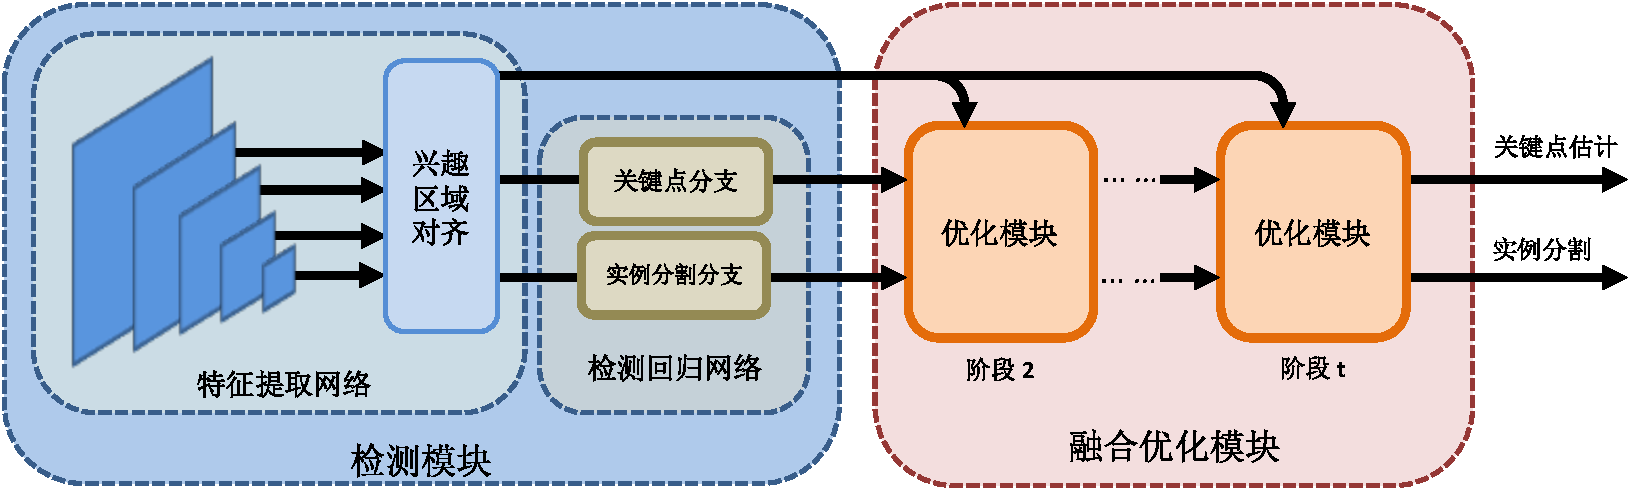
\includegraphics[width=0.8\textwidth]{network.pdf}
	\caption{网络整体结构}
	\label{fig:Overall}
\end{figure*}

%	ROI Extraction
%	key-point & Mask Prdiction
%		Stage One's Prediction
检测模块由特征提取网络与检测回归网络两个模块组成。在特征提取网络中,模型通过特征提取器$E$得到图像$I$来自网络各个尺度的特征$F=\{f_1, f_2, ..., f_5\}$。这些特征被金字塔兴趣区域对齐层$P$\footnote{金字塔兴趣区域对齐层,简称Pyramid RoI Align Layer, 全称Pyramid Region of Interest Align Layer}通过双线性插值的方法对齐至同样的尺寸。每个图像中只有来自特定尺度$k$的特征图$f_k$被选中并被输入至接下来的检测回归网络中。这个被选中的特征被分别送入了实例分割分支$B_m$与姿态估计分支$B_k$,分别得到了实例分割结果$M=\{m^1, m^2, ..., m^n\}$与姿态估计结果$K=\{k^1, k^2, ..., k^n\}$。这些中间结果会被输入到融合优化阶段进行多阶段的回归。为了与融合优化网络中的优化模块输出的名称保持一致,由检测回归网络生成的分割结果$M$与$K$被标记作多阶段中的第一阶段输出$M_1$与$K_1$,这里可以用数学公式描述为:
\begin{equation}
\label{def:detectnet}
M_1, K_1 = B_m(P(E(I))), B_k(P(E(I)))
\end{equation}

%		Stage 2+'s Prediction
在融合优化阶段的第$t(t>2)$阶段,单个优化模块接收来自特征提取器$E$的特征$f_k$、在阶段$t-1$中得到的姿态估计结果$K_{t-1}$与实例分割结果$M_{t-1}$,其中$\otimes$代表张量连接操作。整个网络有主要设计亮点可以归纳为三点。第一是本文引入了注意力机制让网络关注具体的区域,本文设计了注意力转换模块来让生成一个合适的注意力与特征图融合,最后得到关键点预测结果$K_t$。第二,网络还会根据姿态估计的中间结果,也就是一些更偏向于得到关键点预测的特征,生成实例分割的结果。这让网络会根据来自姿态估计的信息修正实例分割的结果。最后,由注意力转换模块生成的注意力还会与从姿态估计那一支生成的中间结果融合,最终生成的实例分割的优化结果$M_t$。因此,整个优化模块$R$可以被抽象为形如:
\begin{equation}
\label{def:refinenet}
M_t, K_t = R(M_{t-1}\otimes f_k, K_{t-1}\otimes f_k)
\end{equation}

%   This part is to describe why we use a hybrid multi-stage arch
%	1. mask and key-point detection is associated
%	2. In crowd, the heatmap is not robust to predict
本方法使用了多阶段、利用弱监督约束的注意力的结构,同时优化实例分割与姿态估计的结果。首先多阶段与中继监督这两个设计可以让网络获得更大的深度,从而得到更多的感受野,让网络能够充分学习关键点之间的关系\cite{wei2016convolutional}。其次,由于实例分割和姿态估计是联系紧密的两个任务,实例分割与姿态估计能够相互优化。该结构设计的主要目标是希望网络能够同时优化姿态估计与实例分割结果。通过引入注意力以及弱监督这种较宽松约束下的可学习参数,网络能够更加适应数据中的不同表现,并且给出具有一定语意的空间注意力\cite{wang2017residual}。这让网络在一些实例分割难以划分实例边界的情况下, 仍然能够生成较为正确的注意力引导关键点的检测与人体骨架的重建。

\section{检测模块}
\label{sec:detectionstage}
%	Structure description
%	1. Hybrid arch of maskrcnn & cpm
本文使用了类似Faster R-CNN\cite{Ren2015Faster}的目标检测器来提取人体位置。本节可以根据检测部分的模块组成分别介绍算法中的设计与实现细节。本节由特征提取网络与检测回归网络两小节组成。

\subsection{特征提取网络}
\label{subsec:featextract}
本文使用了残差网络作为特征提取的基础结构。本文使用了101层残差模块组成的残差网络作为本文方法的特征提取网络,具体ResNet-101的网络结构可以参考图\ref{fig:ResNet}。同时,本文为了更好地融合来自不同尺度的特征,还使用了特征金字塔\cite{Lin2016Feature}来自底向上地融合不同尺寸的特征。构建特征金字塔需要来自基础网络中不同尺寸的特征图。由于网络会使用步长为2的卷积层或池化层每次缩小特征图至原尺寸的1/2,因此在融合不同尺度的特征图时,需要依次上采样两倍以对齐特征图的尺寸。

\begin{figure*}[htbp]	
	\centering
	\begin{subfigure}[b]{0.4\textwidth}
		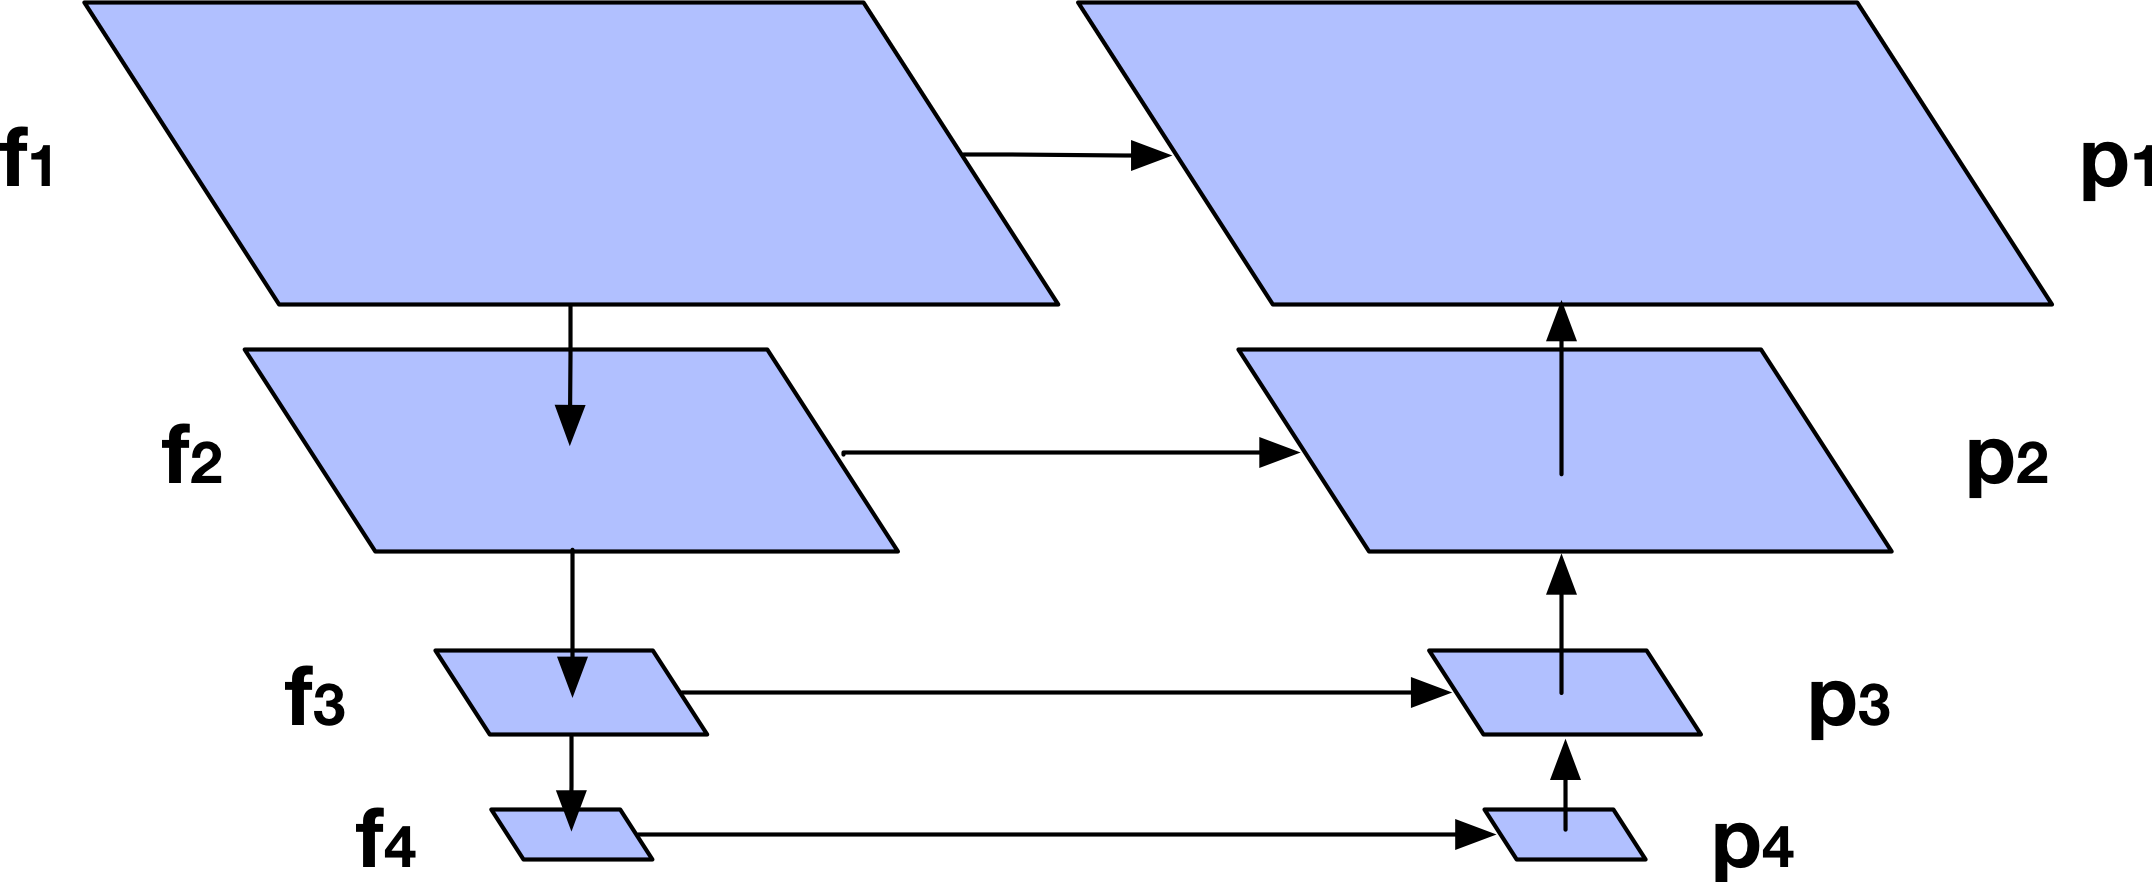
\includegraphics[width=\linewidth]{FPN_a.png}
		\caption{特征金字塔中的特征融合}
	\end{subfigure}
	\hskip1.5cm
	\begin{subfigure}[b]{0.4\textwidth}
		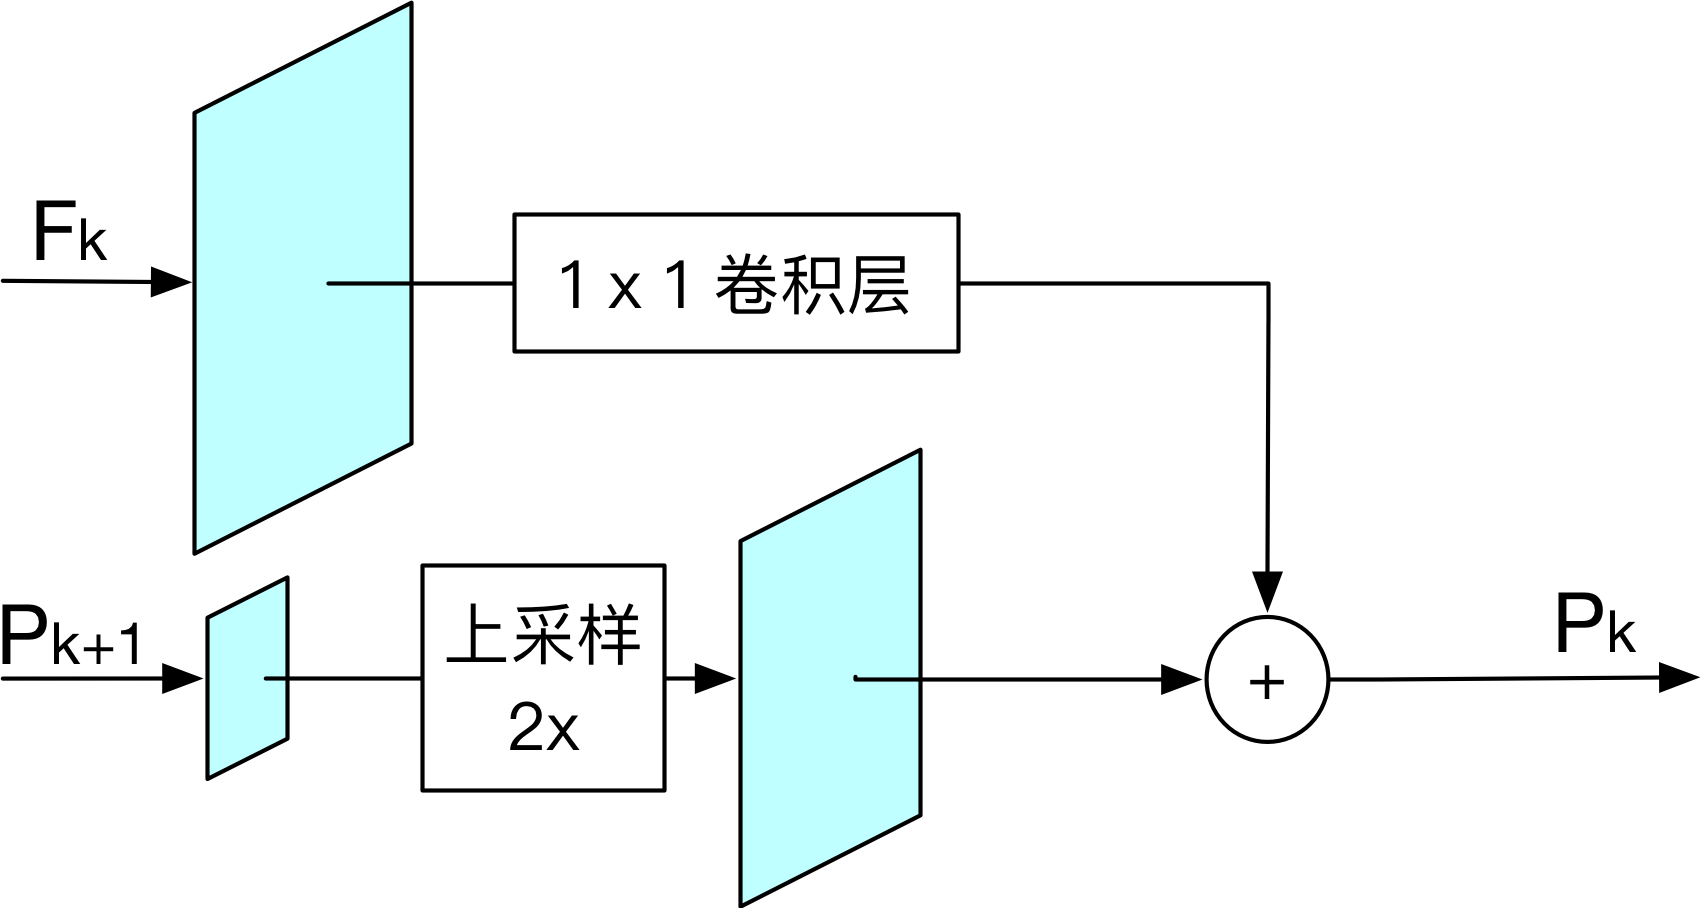
\includegraphics[width=\linewidth]{FPN_b.png}
		\caption{单尺寸特征下的融合结构设计}
	\end{subfigure}
	\caption{特征金字塔中的结构设计}
	\label{fig:FPN}
\end{figure*}

如图\ref{fig:FPN}所示,由残差网络得到的来自不同尺寸的特征图$f_1, f_2, f_3, f_4$会经过特征金字塔的融合得到对应尺度大小的融合特征图$p_1, p_2, p_3, p_4$。对于特定的尺度$k$,特征金字塔会将来自稍小尺度的融合特征$p_{k+1}$与经过1\times1卷积层重新映射的特征图$f_k$相加,得到对应尺度的融合特征图$p_k$。这样特征提取器就可以得到在较为适当的感受野下的特征图。

在使用兴趣区域对齐层裁剪前,本文将所有检测到的边界框调整为正方形,以保持特征的长宽比。在区域对齐层,如果直接输入矩形框作为裁剪依据,那么在对齐尺寸后特征的长宽比将会被破坏,给模型带来性能上的损失。同时,一些不精确的检测结果也许无法涵盖物体的全部区域,这会将检测结果误差传播至接下来的任务中。因此,本文首先将检测框依据最长边的长度由矩形变换为正方形以适应网络期待的输入,同时,再在正方形检测框的外围填补20\%的大小以改善检测结果误差带来的损失。

经过特征金字塔的融合特征图会根据检测到的边界框位置与尺寸被兴趣区域对齐层裁剪并缩放至同一尺寸下。由于这个兴趣区域对齐接收多个尺度的特征图,因此需要设计一种策略来选择与检测结果对应尺度的特征送入检测回归网络。其选择特征的原则可以被描述如下:
\begin{equation}
\label{def:PyramidRoIAlign}
k =\lfloor k_0 + \log_{2}(\sqrt{wh} / 224) \rfloor
\end{equation}
如公式\eqref{def:PyramidRoIAlign}所示,本文设定初始的特征尺度$k_0$为3,而224则是在ImageNet上预训练好的尺寸大小。如果检测结果的面积小于224\times224,那么区域对齐层就会使用尺寸更大的特征裁剪并缩放;反之,如果检测结果的面积更大,对齐层则会选择尺寸更小,感受野相对更大的特征作为裁剪的对象。最终,被裁剪对齐的特征被分别被送入检测回归网络与融合优化网络中作为回归关键点与分割结果的依据。

\subsection{检测回归网络}
\label{subsec:detection}
检测回归网络是由两个并行的分支组成的。实例分割分支与姿态估计分支分别使用裁剪好的特征得到粗略的实例分割结果与姿态估计结果。分割分支的网络结构采用了类似Mask R-CNN\cite{He2017Mask}的子网结构,使用了四层3\times3卷积层,和一层1\times1的卷积层。类似地,姿态估计分支使用了五层卷积核大小为3的卷积层,最终的输出被两层1\times1卷积调整至关键点外加背景个通道,以得到每个关键点的热力图。两个分支的输出尺寸完全匹配,并且每个像素在空间关系上一一对应。在检测回归网络中,两个分支都是以并行方式计算的。两个任务并不会在特征层面上进行融合。本模块的设计目的就是为融合优化提供一个更好的初始状态。为了与融合优化网络输出命名保持一致,检测回归网络的实例分割输出与关键点预测输出被分别定义为$M_1$与$K_1$。

\section{融合优化网络}
\label{sec:refine}
本文使用了多个具有相同结构的优化模块同时优化实例分割与姿态估计结果。新提出的优化模块引入了软注意力来强化对应区域的特征响应,从而优化网络在遮挡情况下对于单人结构的理解。并且软注意力还会用来增强实例分割的特征表达,将分割信息在模块间相互传递并优化。

\subsection{优化模块结构设计}
\label{subsec:architecture}

优化模块结构设计如图\ref{fig:RefineNet}所示。优化模块的设计有两个目标,一个是将多任务的每个分支的信息从当前阶段传递到下一个阶段;另一个目标是网络应该有较好的融合方法让两个任务的特征。对于第一个目标,网络结构在每个分支都设计了传递的结构,以增强每个阶段在现有结果上优化的能力;其次,本文对于两个任务特征融合也对应设计了融合方法以达到交叉优化的目标。所以本文提出了涉及了多个拥有相同结构的优化模块多阶段地融合关键点信息与分割信息以增强姿态估计与实例分割的最终结果。

\begin{figure*}[h]	
	\centering
	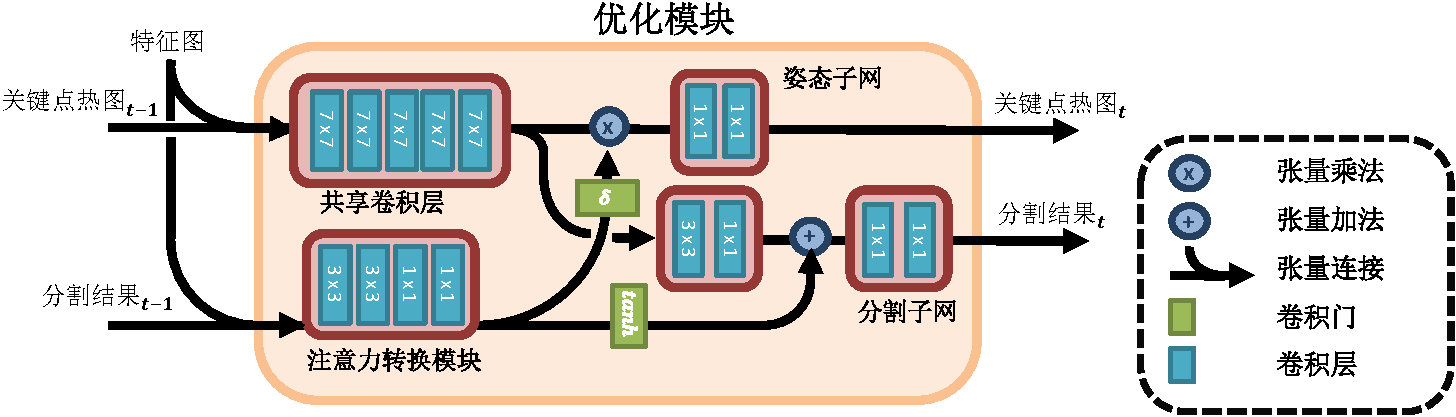
\includegraphics[width=0.8\textwidth]{RefineNet.pdf}
	\caption{融合优化模块具体设计}
	\label{fig:RefineNet}
\end{figure*}

每一个优化模块可以被抽象地定义为公式\eqref{def:refinenet}。首先,优化模块会把输入的特征分为两部分。第一份拷贝$f$会首先与来自阶段$t-1$的姿态结果$K_{t-1}$进行合并,并一同被送入一组共享的卷积层$C$中,得到姿态特征图$c$,如公式\eqref{def:sharedconv}\footnote{公式中的$\otimes$代表张量连接操作。}所示。第二份特征图拷贝$f$同样会与上一阶段的实例分割结果$M_{t-1}$进行合并,并被输入至注意力转换模块$A$中,得到注意力特征图$a$,如公式\eqref{def:attenconverter}\footnote{公式中的$\odot$代表张量内积操作。}所示。如公式\eqref{def:keypointhead}所描述,之后姿态特征图$c$会与经过$\sigma$门\footnote{$\sigma$门由一组神经层和一个$sigmoid$激活函数组成,会将网络输出限制在$[0,1]$的值域中}重新映射的注意力$a_s$相乘,经过姿态子网$H_k$的调整,最终输出关键点预测结果$K_t$。这样的设计让网络能够根据实例分割的结果生成注意力,让网络根据生成的注意力$a$生成更加鲜明的姿态估计结果。

\begin{equation}
\label{def:sharedconv}
c = C(f\otimes{K_{t-1}})
\end{equation}
\begin{equation}
\label{def:attenconverter}
a = A(f\otimes{M_{t-1}})
\end{equation}
\begin{equation}
\label{def:keypointhead}
K_t = H_k(c\odot \sigma(a))
\end{equation}

由注意力转换模块生成的注意力特征图$a$,不但会影响关键点预测的结果$K_t$,还会影响实例分割的结果$M_t$。如公式\eqref{def:fusion}所示,首先网络会利用来自共享卷积层的姿态特征图$c$经过一组3\times3卷积层$F$生成一组供实例分割使用的特征图。这组特征图接下来会与经过$\tanh$门\footnote{$\tanh$门由一组神经层和一个$\tanh$激活函数组成,会将网络输出限制在$[-1, 1]$的值域中。}调整的注意力$a_{\tanh}$相加,融合了来自注意力转换模块的信息,共同送入分割子网$H_s$得到最终优化的分割结果$M_t$。

\begin{equation}
\label{def:fusion}
M_t = H_m(F(c) \oplus \tanh(a))
\end{equation}

总而言之,网络的整体设计可以被概括为两部分:传递与交叉。姿态估计的传递方法很简单,是直接经过特征图传递的。但在传递实例分割信息的时候,过程就稍显复杂一些:网络使用从注意力调整模块生成的注意力$a_k$,与从姿态估计分支得到的特征图相加而完成对分割信息的多阶段传递。经过加和的部分同样会被注意力强化,只不过相比于乘性强化而言,加性强化并不会减弱特征信息的表达,仅仅是完成了特征的融合。因为在实例分割部分,我们并不希望减弱对应区域的特征,而仅仅希望是引入上一阶段的结果信息而已。

交叉过程的核心就是本文引入的注意力机制。在姿态估计方面,网络使用注意里调整模块生成的注意力完成向姿态估计任务引入分割信息的过程。因为本文定义的注意力调整模块不仅会接收来自特征提取器的特征图,还会接收来自上一阶段的分割结果图。这意味着分割结果图的预测结果会影响姿态估计结果的生成。另外在实例分割的部分,网络使用来自姿态分支特征图与注意力相加来完成交叉优化的目标。最终,两个分支通过涵盖两任务特征传递与特征交叉的设计完成了交叉优化的目标。

为了设计更加合适的约束,算法应该同时监督每个阶段优化模块的两个输出:实例分割结果$S$与姿态估计结果$K$。本文希望通过显式监督两个现有任务的方式,内隐地得到适合数据的注意力的生成方式。由于现在对于实例分割与姿态估计两个任务的监督方法已经相当成熟,所以这两个监督信息应该能够提供足够的约束来得到能够有较强语义的空间注意力。

\begin{figure}[ht]
	\centering
	\begin{subfigure}[b]{0.18\linewidth}
		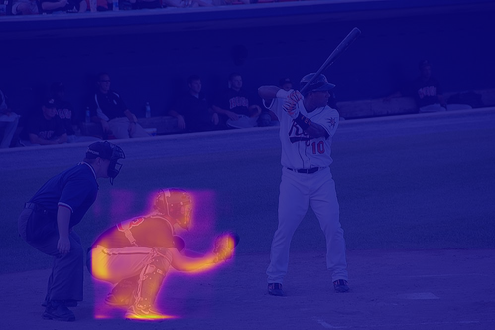
\includegraphics[width=\linewidth]{6471_insid1_stage1_atten.PNG}
		\caption{阶段2}
	\end{subfigure}
	\begin{subfigure}[b]{0.18\linewidth}
		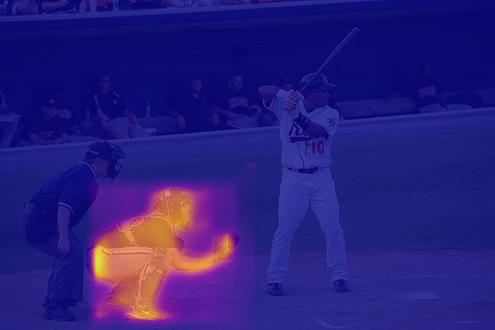
\includegraphics[width=\linewidth]{6471_insid1_stage2_atten.PNG}
		\caption{阶段3}
	\end{subfigure}
	\begin{subfigure}[b]{0.18\linewidth}
		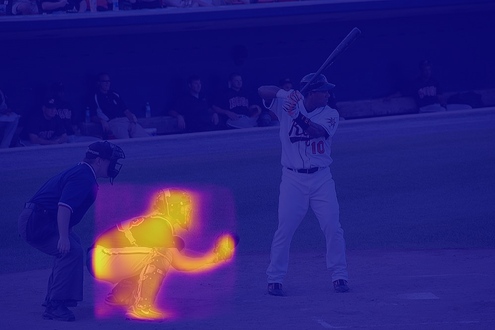
\includegraphics[width=\linewidth]{6471_insid1_stage3_atten.PNG}
		\caption{阶段3}
	\end{subfigure}
	\begin{subfigure}[b]{0.18\linewidth}
		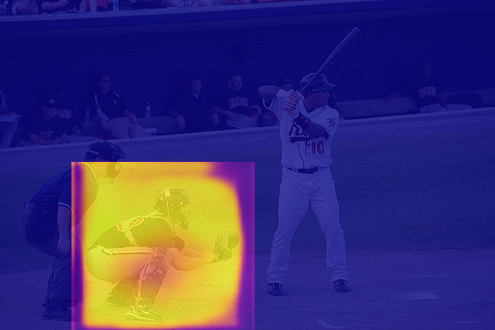
\includegraphics[width=\linewidth]{6471_insid1_stage4_atten.PNG}
		\caption{阶段4}
	\end{subfigure}
	\begin{subfigure}[b]{0.18\linewidth}
		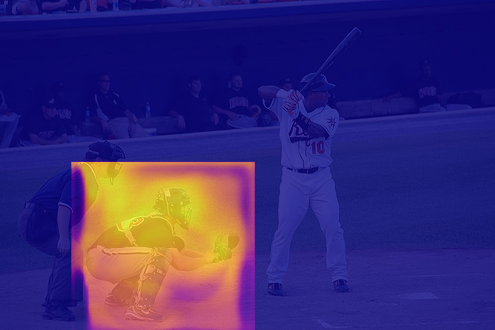
\includegraphics[width=\linewidth]{6471_insid1_stage5_atten.PNG}
		\caption{阶段5}
	\end{subfigure}
	\caption{多阶段的优化模块堆叠会导致关键点分支无法提供足够的监督信息}
	\label{fig:multistageattention}
\end{figure}

如图\ref{fig:attention_mask}所示,在验证实验中本文发现,虽然一定的优化模块能够优化注意力细化需要关注的区域,但过多的优化模块并不会对两任务继续起到联合优化的作用。这可能是因为在单人姿态估计网络中,如图\ref{fig:singleposemultistage}中所展示,更多堆叠卷积层带来的大感受野已经使网络获得分辨人体的能力。这将使注意力的生成失去足够的监督信息而无法学习到在多人场景中区分实例的方法。因此在本文提出的更多阶段优化策略中,选择在阶段4以后停止使用优化模块,取而代之使用类似CPM\cite{wei2016convolutional}中由$7\times7$卷积层构成的回归模块替换优化模块。为了将这一策略与上文提到的基础方法有所区分,本文将网络后面使用额外+号来将4阶段(本文方法)与上文提到的改良6阶段模型(本文方法+)区别开来。

\begin{figure}[h]
\centering
\begin{subfigure}[b]{0.2\linewidth}
	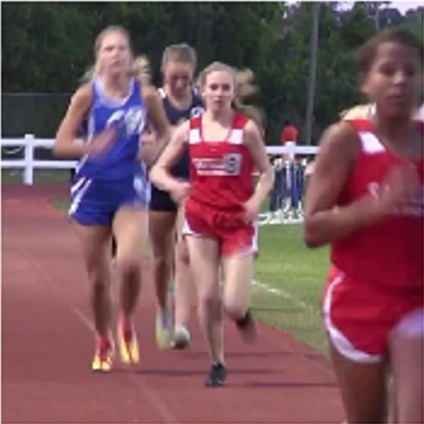
\includegraphics[width=\linewidth]{MPII_multi-stage-single_image.PNG}
	\caption{输入图像}
\end{subfigure}
\begin{subfigure}[b]{0.2\linewidth}
	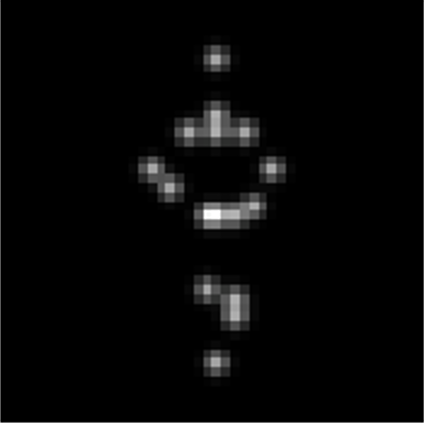
\includegraphics[width=\linewidth]{MPII_multi-stage-single_GT.PNG}
	\caption{真值热图}
\end{subfigure}
\begin{subfigure}[b]{0.2\linewidth}
	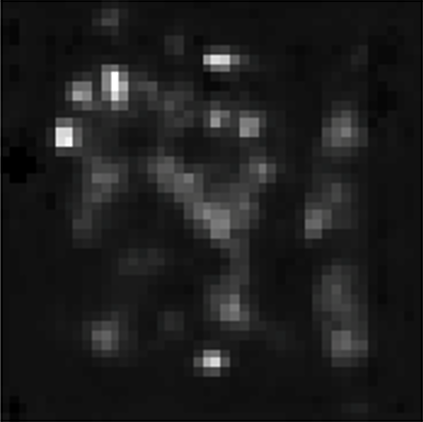
\includegraphics[width=\linewidth]{MPII_multi-stage-single_stage1.PNG}
	\caption{阶段1}
\end{subfigure}
\begin{subfigure}[b]{0.2\linewidth}
	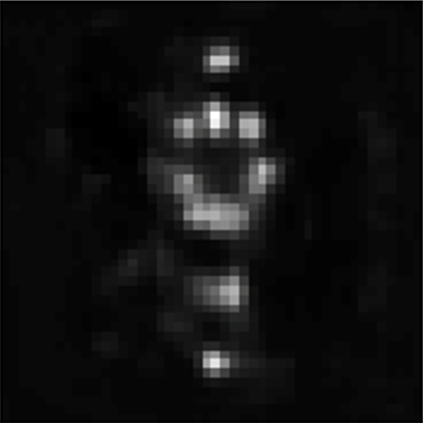
\includegraphics[width=\linewidth]{MPII_multi-stage-single_stage2.PNG}
	\caption{阶段2}
\end{subfigure}

\begin{subfigure}[b]{0.2\linewidth}
	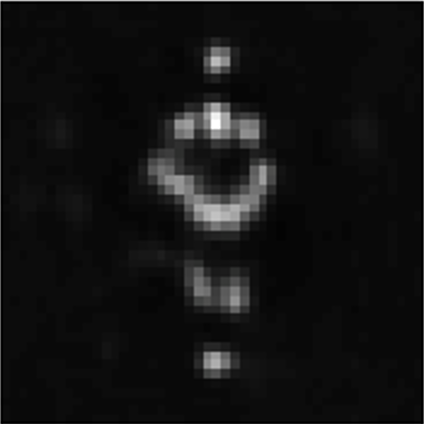
\includegraphics[width=\linewidth]{MPII_multi-stage-single_stage3.PNG}
	\caption{阶段3}
\end{subfigure}
\begin{subfigure}[b]{0.2\linewidth}
	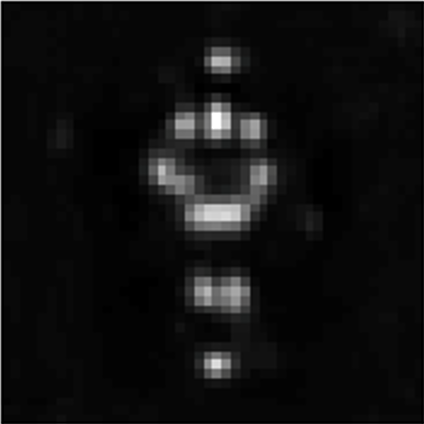
\includegraphics[width=\linewidth]{MPII_multi-stage-single_stage4.PNG}
	\caption{阶段4}
\end{subfigure}
\begin{subfigure}[b]{0.2\linewidth}
	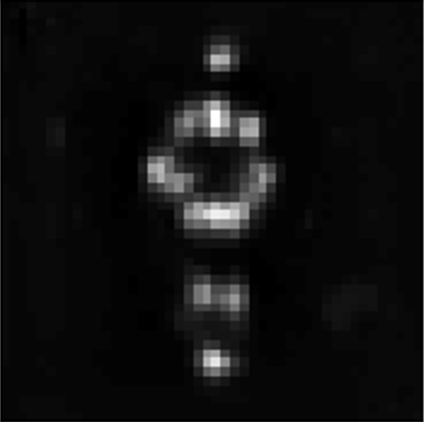
\includegraphics[width=\linewidth]{MPII_multi-stage-single_stage5.PNG}
	\caption{阶段5}
\end{subfigure}
\begin{subfigure}[b]{0.2\linewidth}
	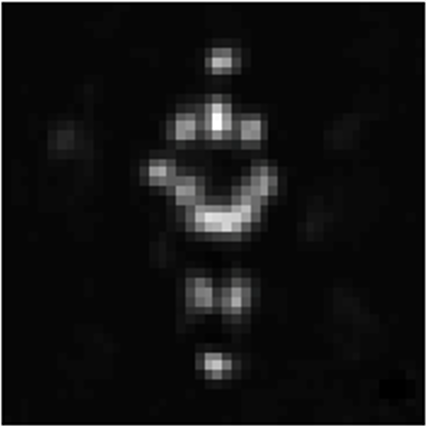
\includegraphics[width=\linewidth]{MPII_multi-stage-single_stage6.PNG}
	\caption{阶段6}
\end{subfigure}
\caption{深度网络下的单人姿态估计网络也可以较好地分辨被选中的实例}
\label{fig:singleposemultistage}
\end{figure}

\subsection{弱监督与注意力机制}
\label{subsec:weaksuper_attention}

本文特别将注意力点乘的部分设计到了$1\times1$卷积之前,而不是简单的在模块开始。由于即大卷积核下的卷积操作会囊括更多的邻近区域信息,导致经过空间注意力重新选择的特征在空间结构上被破坏,因此本文选择了在$k\times k$卷积之前的注意力点乘以使生成的空间注意力直接作用于输出特征的空间位置上。这样能够保证网络输出足够稳定,并且在监督过程中也不会出现其他影响在弱监督条件下约束的注意力生成的因素。

\begin{figure}[h]
	\centering
	\begin{subfigure}{0.23\textwidth}
		\centering
		\begin{subfigure}[b]{\linewidth}
			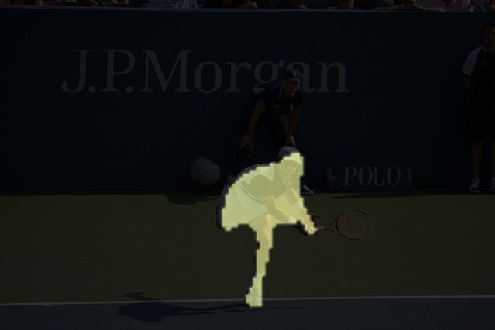
\includegraphics[width=\linewidth]{885_insid0_stage3_mask.png}
		\end{subfigure}
		\vskip2pt
		\begin{subfigure}[b]{\linewidth}
			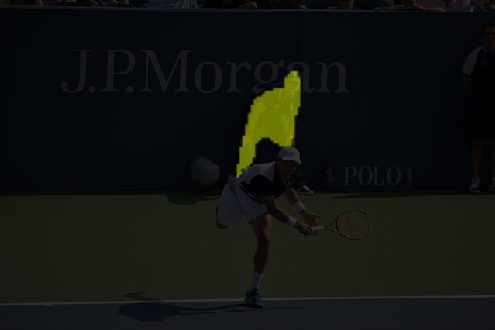
\includegraphics[width=\linewidth]{885_insid1_stage3_mask.png}
		\end{subfigure}
		\caption{分割信息}
	\end{subfigure}
	\begin{subfigure}{0.23\textwidth}
		\begin{subfigure}[b]{\linewidth}
			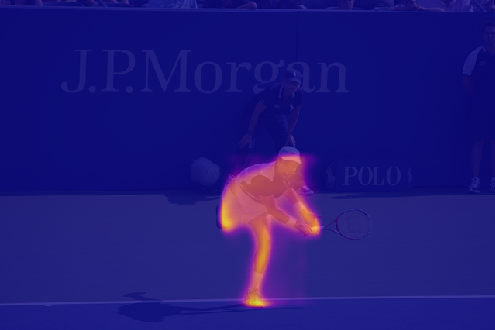
\includegraphics[width=\linewidth]{885_insid0_stage1_atten.png}
		\end{subfigure}
		\vskip2pt
		\begin{subfigure}[b]{\linewidth}
			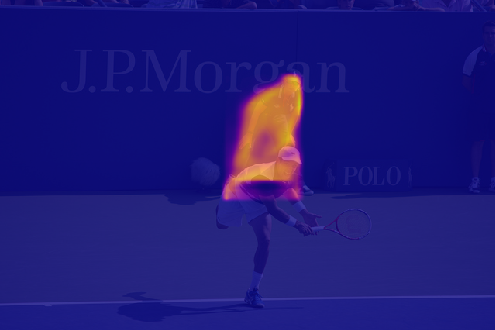
\includegraphics[width=\linewidth]{885_insid1_stage1_atten.png}
		\end{subfigure}
		\caption{阶段2注意力}
	\end{subfigure}
	\begin{subfigure}{0.23\textwidth}
		\begin{subfigure}[b]{\linewidth}
			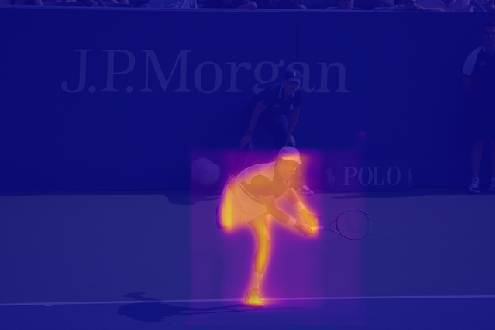
\includegraphics[width=\linewidth]{885_insid0_stage2_atten.png}
		\end{subfigure}
		\vskip2pt
		\begin{subfigure}[b]{\linewidth}
			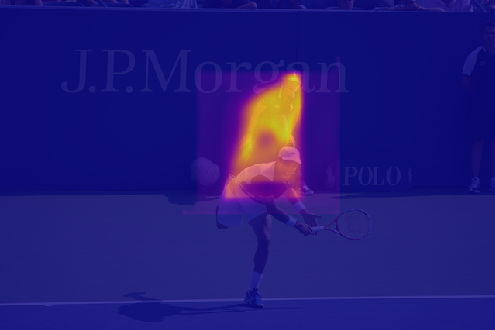
\includegraphics[width=\linewidth]{885_insid1_stage2_atten.png}
		\end{subfigure}
		\caption{阶段3注意力}
	\end{subfigure}
	\begin{subfigure}{0.23\linewidth}
		\centering
		\begin{subfigure}[b]{\linewidth}
			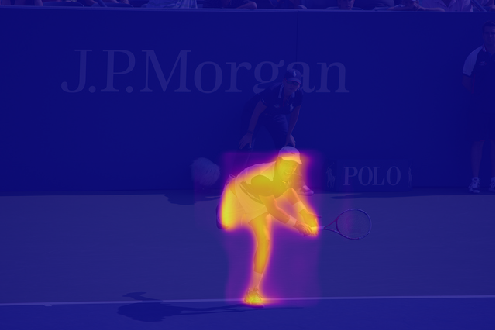
\includegraphics[width=\linewidth]{885_insid0_stage3_atten.png}
		\end{subfigure}
		\vskip2pt
		\begin{subfigure}[b]{\linewidth}
			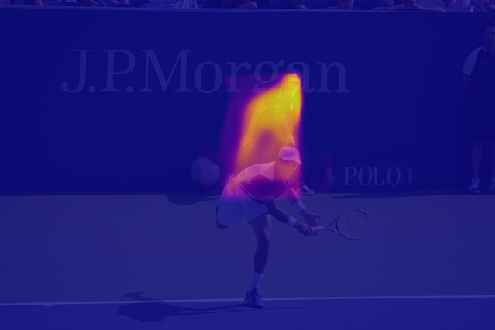
\includegraphics[width=\linewidth]{885_insid1_stage3_atten.png}
		\end{subfigure}
		\caption{阶段4注意力}
	\end{subfigure}
	\begin{minipage}{0.05\linewidth}
		\rotatebox[origin=lt]{90}{\centering 遮挡人}
		
		\vskip1cm
		\rotatebox[origin=lt]{90}{\centering 被遮挡人}
	\end{minipage}
	\caption{空间注意力能够提供比分割信息更多的划分区域}
	\label{fig:attention_mask}
\end{figure}

本文在选取注意力的表现形式时,使用了软注意力作为交叉优化中媒介。实际上,实例分割的结果可以被当做一种注意力。因为使用分割结果在网络后处理阶段直接进行点乘处理,即在关键点热图使用分割结果做遮罩操作,在简单的融合实例分割信息的多人姿态估计策略中是很常见的。这种处理就相当于强化了对应空间位置的热图响应,与注意力的机理十分相似的。虽然实例分割也是网络自生成的结果,但由于其并不能考虑遮挡部分的人体区域。单独设计的注意力转换器能够在宽松的实例分割信息监督影响下生成对遮挡部分区域的响应。另外,实例分割结果是二值化图像,相当于一种硬注意力。如图\ref{fig:attention_mask}所示,与软注意力相比,硬注意会直接消除特征图对应位置的特征响应,损失了很多网络预测关键点位置所依赖的特征。并且这样使用硬注意力的系统会受限制于硬注意力本身,一旦生成的硬注意力不准确,就会在像姿态估计这种对于精确度要求很高的任务上失败。在Wang的工作\cite{wang2017residual}中也使用了软注意力来完成图像分类这一精度要求较高的任务,他们使用单独的分支生成注意力以增强对应区域的特征响应。这充分说明了软注意力在完成精确任务的目标上是必须的。

本文提出的优化模块主要可以让两个任务互相交叉优化:第一,姿态估计会向实例分割提供特征图,优化实例分割结果,如公式\eqref{def:fusion}。第二就是来自实例分割的特征会融合进入姿态子网对姿态估计结果进行优化,如公式\eqref{def:keypointhead}。其中第一点比较好实现,因为可以直接设计从姿态估计过程中抽取中间特征图来生成实例分割结果,就如公式\eqref{def:fusion}中的$F$的作用一样。

对于第二点中使用分割信息优化姿态结果的任务,本文使用弱监督学习下生成的空间注意力来优化姿态估计结果。如果使用强监督学习,那么在实例分割信息监督下生成的注意力将无法完整地勾勒人体边界。如图\ref{fig:attention_mask}所示,实例分割监督信息不会考虑遮挡情况下的躯干边界。同时,即使现有条件能够满足重新补全标注信息以满足任务要求,数据也不能保证整齐准确。因为使用人工的方式得到被遮挡躯干的轮廓不仅要消耗比简单分割标定更多的时间,还会因为这个任务过强的主观性导致标定数据的偏差很大,难以获得较为稳定的标定结果。这会导致网络无法在这样标定的数据下很好地收敛。因此,在这样的情况下,网络需要更加宽松的约束来监督注意力的生成。根据Zhou对于弱监督学习的总结\cite{10.1093/nsr/nwx106},弱监督学习可以在监督学习不准确、不完整的情形下,给出相对准确完整的预测信息。而本文的目标正是希望借助不完整的实例分割信息生成补全被遮挡人体部位的区域响应。因此本文必须使用弱监督学习来达成这一目标。

在如何将注意力携带的传递到下一阶段的方案上,本文的最初目的就是改善本阶段的特征表达,以生成更好地实例分割结果。之所以在这个位置设计$\tanh$门来调整输出范围,是因为注意力不仅能够影响特征注意区域,也能够帮助特征强化对应位置。另外,最终生成的经过$\tanh$门映射的注意力$a_{\tanh}$也携带着上一阶段的信息,因此也是有必要将这一部分信息与生成的实例分割特征融合。于是本文希望借助一个变型的残差网络,使用张量加法将生成的注意力$a_{\tanh}$融合输入到分割子网,得到了最终的实例分割结果。


\section{网络训练}
\label{sec:training}
\subsection{损失函数}
\label{subsec:lossfunction}
%	Section 2 Training
%	key-point Loss
%	Why Applying masks after 1x1 conv?
%	1.	explicitly define loss with mask & key-points
%	2.	simply enhance response of the heatmap
%		rather than enhance the result
%			--> This will give more responses

本文监督网络的损失函数可以被分为三部分:边界框损失函数、关键点分支损失函数与实例分割损失函数,如公式\eqref{detection_loss}。为了平衡每个分支的收敛速率,本文设计了$\beta$和$\alpha$分别控制目标检测与实例分割的损失函数权重。对于目标检测监督与实例分割监督而言,损失函数的设计与选择已经相当成熟。如公式\eqref{mask_loss}与公式\eqref{bbox_loss}所示,损失函数在这里使用类似Fast R-CNN\cite{Girshick2015Fast}的交叉熵来度量真实标签与预测向量的差距。只不过与目标检测的损失函数$L_{bbox}$定义不一样,实例分割的损失函数$L_{mask}$是以多阶段中继监督的形式体现出来的。在本文的实验中为了方便操作,暂时将$\beta$设置为0同时固定预训练的检测模块的参数。通过将$\alpha$设置为0.1来强化实例分割对于网络整体训练的影响。本文使用了加入中级监督的类似L2范数形式来定义姿态估计分支的损失函数\eqref{key-point_loss}。对于优化模块而言,实例分割与姿态估计两个的任务的损失函数会同时作用于网络自生成的注意力上。这样既能够达到本文最初训练能够完成多任务的优化模块的目标,又能够让网络得到一个更加适应数据的注意力。而通过这样的监督方法,也希望能够证明,适应数据的注意力也能够在语义性上具有较强的可解释性。

\begin{align}
L_{total} &= \beta L_{bbox} + \alpha L_{mask} + L_{key-point}\label{detection_loss}\\
L_{bbox} &= -\sum_{c \in C}{\hat{p_c} \log{p_c^{*}}}\label{bbox_loss}\\
L_{mask} &= -\sum_{t=1}^{T}\sum_{c \in C}{\hat{s_c} \log{s_c^{*}}}\label{mask_loss}\\
L_{key-point} &= \sum_{t=1}^{T}\sum_{i \in I}\sum_{k \in K}{\left\| \hat{k_i} - {k_i}^{*} \right\|_2}\label{key-point_loss}
\end{align}

\subsection{梯度分析}
\label{subsec:gradient}
本文提出的优化模块结构涉及到两支输出相互交叉与传递,因此本文需要给出对应损失函数对于梯度的影响,从而证明网络能够在添加结构的条件下保证两支网络的正常收敛。分析梯度主要是通过对网络求导来完成。因为在梯度回传过程中需要计算输入对输出的导数,通过将本层导数与来自上层的梯度相乘,可以得到本层的参数更新梯度。因此,通过对网络求导方式,可以更加直观地分析梯度回传的大小,从而改善网络收敛的特性。尤其对于多任务融合网络而言,为了让网络最优,梯度分析更加重要。

为了方便求导,不妨设$f \otimes K_{t-1}$为$X^k_{t-1}$,$f \otimes M_{t-1}$为$X^m_{t-1}$。同时,引用公式\eqref{def:sharedconv}、公式\eqref{def:attenconverter}、公式\eqref{def:fusion}以及公式\eqref{def:keypointhead}中的符号,那么损失函数对优化模块的输入$X^k_{t-1}$与$X^m_{t-1}$的影响程度可以被分别推导为:
\begin{corollary}
\label{corollary:loss2xk}
全局损失$L$函数对优化模块的输入$X^k_{t-1}$的求导:
\begin{equation*}
\begin{aligned}
\frac{\partial L}{\partial X_{t-1}^k} &= \frac{\partial L}{\partial M_t}\frac{\partial M_t}{\partial X_{t-1}^k} + \frac{\partial L}{\partial K_t}\frac{\partial K_t}{\partial X_{t-1}^k}\\
&= \frac{\partial L}{\partial M_t}\frac{\partial M_t}{\partial H_m}\frac{\partial H_m(c)}{\partial X_{t-1}^k} + \frac{\partial L}{\partial K_t}\frac{\partial K_t}{\partial ca_{\sigma}}\frac{\partial ca_{\sigma}}{\partial X_{t-1}^k}\\
&= \frac{\partial L}{\partial M_t}\frac{\partial M_t}{\partial H_m(c)}\frac{\partial H_m(c)}{\partial c}\frac{\partial c}{\partial X_{t-1}^k} + a_{\sigma}\frac{\partial L}{\partial K_t}\frac{\partial K_t}{\partial ca_{\sigma}}\frac{\partial c}{\partial X_{t-1}^k}
\end{aligned}
\end{equation*}
\end{corollary}
\begin{corollary}
\label{corollary:loss2xm}
全局损失$L$函数对优化模块的输入$X^m_{t-1}$的求导:
\begin{equation*}
\begin{aligned}
\frac{\partial L}{\partial X^m_{t-1}} &= \frac{\partial L}{\partial M_t}\frac{\partial M_t}{\partial X^m_{t-1}} + \frac{\partial L}{\partial K_t}\frac{\partial K_t}{\partial X^m_{t-1}}\\
&=\frac{\partial L}{\partial M_t}\frac{\partial M_t}{\partial a_{\tanh}}\frac{\partial a_{\tanh}}{\partial X^m_{t-1}} + \frac{\partial L}{\partial K_t}\frac{\partial K_t}{\partial ca_{\sigma}}\frac{\partial ca_{\sigma}}{\partial X^m_{t-1}}\\
&=\frac{\partial L}{\partial M_t}\frac{\partial M_t}{\partial a_{\tanh}}\frac{\partial a_{\tanh}}{\partial a}\frac{\partial a}{\partial X^m_{t-1}} + c\frac{\partial L}{\partial K_t}\frac{\partial K_t}{\partial ca_{\sigma}}\frac{\partial a_{\sigma}}{\partial X^m_{t-1}}
\end{aligned}
\end{equation*}
\end{corollary}

同时根据在公式\eqref{detection_loss}全局损失的定义,所以损失函数对于分割分支的输出影响可以被可以被推导为:
\begin{equation*}
\begin{aligned}
\frac{\partial L}{\partial M_t} &= \frac{\partial (\alpha L_{mask} + L_{key-point})}{\partial M_t}\\
&= \alpha\frac{\partial L_{mask}}{\partial M_t} + \frac{\partial L_{key-point}}{\partial M_t}
\end{aligned}
\end{equation*}

根据公式\eqref{key-point_loss}中定义,关键点损失函数仅与关键点输出$K$有关,因此不难得出$\frac{L_{key-point}}{\partial M_t}=0$。那么在上文中陈述的推导过程中,全局损失函数对于分割分支的输出影响可以被化简为:
\begin{equation}
\label{eq:L2Mt}
\frac{\partial L}{\partial M_t} = \alpha\frac{\partial L_{mask}}{\partial M_t}
\end{equation}
同样地,根据公式\eqref{mask_loss}中定义,分割任务损失也仅与分割输出$M$有关,故不难得出$\frac{L_{mask}}{\partial K_t}=0$。那么全局损失函数对于关键点分支的输出影响同样可以被推导为
\begin{equation}
\label{eq:L2Kt}
\frac{\partial L}{\partial K_t} = \frac{\partial L_{key-point}}{\partial K_t}
\end{equation}

结合推论\ref{corollary:loss2xk}与推论\ref{corollary:loss2xm}和公式\eqref{eq:L2Kt}与公式\eqref{eq:L2Kt},不难得出全局损失函数中的不同部分对于不同分支输入的影响:
\begin{align}
\frac{\partial L_{key-point}}{\partial X^k_{t-1}} &= a_{\sigma}\frac{\partial L}{\partial K_t}\frac{\partial K_t}{\partial ca_{\sigma}}\frac{\partial c}{\partial X_{t-1}^k}\label{def:dloss_keyloss-key}\\
\frac{\partial L_{key-point}}{\partial X^m_{t-1}} &= c\frac{\partial L}{\partial K_t}\frac{\partial K_t}{\partial ca_{\sigma}}\frac{\partial a_{\sigma}}{\partial X^m_{t-1}}\label{def:dloss_keyloss-mask}\\
\frac{\partial L_{mask}}{\partial X^k_{t-1}} &= \alpha\frac{\partial L}{\partial M_t}\frac{\partial M_t}{\partial H_m(c)}\frac{\partial H_m(c)}{\partial c}\frac{\partial c}{\partial X_{t-1}^k}\label{def:dloss_maskloss-key}\\
\frac{\partial L_{mask}}{\partial X^m_{t-1}} &= \alpha\frac{\partial L}{\partial M_t}\frac{\partial M_t}{\partial a_{\tanh}}\frac{\partial a_{\tanh}}{\partial X^m_{t-1}}\label{def:dloss_maskloss-mask}
\end{align}
其中,公式\eqref{def:dloss_keyloss-key}描述关键点信息对于关键点分支输入的影响;公式\eqref{def:dloss_keyloss-mask}描述了关键点监督信息对于优化模块下支输入的影响。同样地,分割损失函数对于上下支的影响也可以分别描述为公式\eqref{def:dloss_maskloss-key}与公式\eqref{def:dloss_maskloss-mask}。

可以看到在公式\eqref{def:dloss_keyloss-key}与公式\eqref{def:dloss_keyloss-mask}中看到,关键点部分损失函数会同时影响到优化模块的两个输入。但由于损失函数对于上下两支的影响会分别受到中间输出$c$与$a_{\sigma}$的影响,因此本文使用了L2正则化让$c$的输出尽可能小,使从关键点损失回传的梯度变小,从而相对减小关键点信息对于分割信息的影响,也就意味着关键点损失会对注意力转换器中参数的影响被削弱。相反地,因为本文希望增强关键点损失对于共享卷积层的影响,所以本文使用带负号的L2正则化使$a_{\sigma}$的输出更倾向于远离0,从而让对应损失函数对于对应分支的影响增大,让关键点损失更多地将梯度回传进入共享卷积层。

同样地,在公式\eqref{def:dloss_maskloss-key}与公式\eqref{def:dloss_maskloss-mask}中,分割损失函数也会同时影响进入优化模块的两支输入。不同的是,分割损失函数并不会由于任何中间结果受到影响,因此本文没有涉及特殊策略平衡分割任务损失函数对于不同分支的梯度影响。


\subsection{训练策略}
\label{subsec:trainingstrategy}

本文在训练过程中使用数据扩增技术让网络获得更好泛化性。本文使用了旋转、缩放和检测框抖动技术来对数据进行扩增。本文在$[-30^\circ, +30^\circ]$的范围内随机选取角度同时对训练数据与输入特征进行旋转。同时,本文还在$[0.7, 1.3]$范围内随机选取比例对训练数据与输入特征进行缩放,缩放使用双线性插值进行对尺寸的调整。最终,为了保证网络对于不准确检测结果的适应性,本文对训练用的目标框进行了随机抖动扩增。在本节中所有的随机方式输出都服从高斯分布。

本文使用了两阶段的训练策略来监督整个网络。在第一阶段,先训练检测部分使用对应部分的损失函数进行训练至大致收敛,接着加入融合优化部分的多阶段优化模块使用整体损失函数进行监督。在第一阶段的检测网络训练策略上,仅针对目标检测损失函数进行训练,学习率为0.05,并采取学习率阶梯下降的方法,间隔30代下降一次学习率,每次下降的系数为0.5。在样本批为8的设定下整体训练120代,其中代长为1000步。在第二阶段的训练中,训练策略主要倾向于优化融合优化的部分。对网络整体损失函数的学习率被设定为0.0005,间隔60代下降一次学习率,学习率下降策略同样采取阶梯式,每次下降系数为0.333。网络在批大小为1的条件下整体训练200代,其中代长为1000步。

由于本文中涉及到多个不同任务的监督信息,因此需要更加复杂的训练策略监督网络的收敛。在网络训练中,要极力避免损失函数中的不同项之间的竞争。因此本文在训练过程中,为了消除这种可能的竞争情况,将检测部分抽出单独监督。在完成对检测网络的训练之后,也就是损失函数在收敛至较小的情况下,加入姿态估计与实例分割的损失函数进行监督,让损失函数尽可能多地监督这两个任务,而不是被过大的其他项所限制,导致网络难以收敛。

\section{本章小结}
本章在章节\ref{sec:methodoverview}陈述了算法的整体网络结构。同时本文提出了一种新结构来同时融合优化实例分割与姿态估计两个任务。这种新结构有两个设计目标:传递与交叉。换言之,就是要求这种结构能够融合来自上阶段的中间结果进行估计,同时还要让姿态估计与实例分割任务交叉优化。考虑到以上的两点目标,本文引入了使用弱监督约束的软注意力来连接两个分支的信息,使网络能够使用来自两个分支的信息分别完成两个任务的估计。这样的结构设计不仅强化网络对于单人姿态的理解,也增强了实例分割中网络对于特征的表达。